\section{moLSCheckPoint$<$ M $>$ Class Template Reference}
\label{classmo_l_s_check_point}\index{moLSCheckPoint@{moLSCheckPoint}}
Class which allows a checkpointing system.  


{\tt \#include $<$moLSCheckPoint.h$>$}

Inheritance diagram for moLSCheckPoint$<$ M $>$::\begin{figure}[H]
\begin{center}
\leavevmode
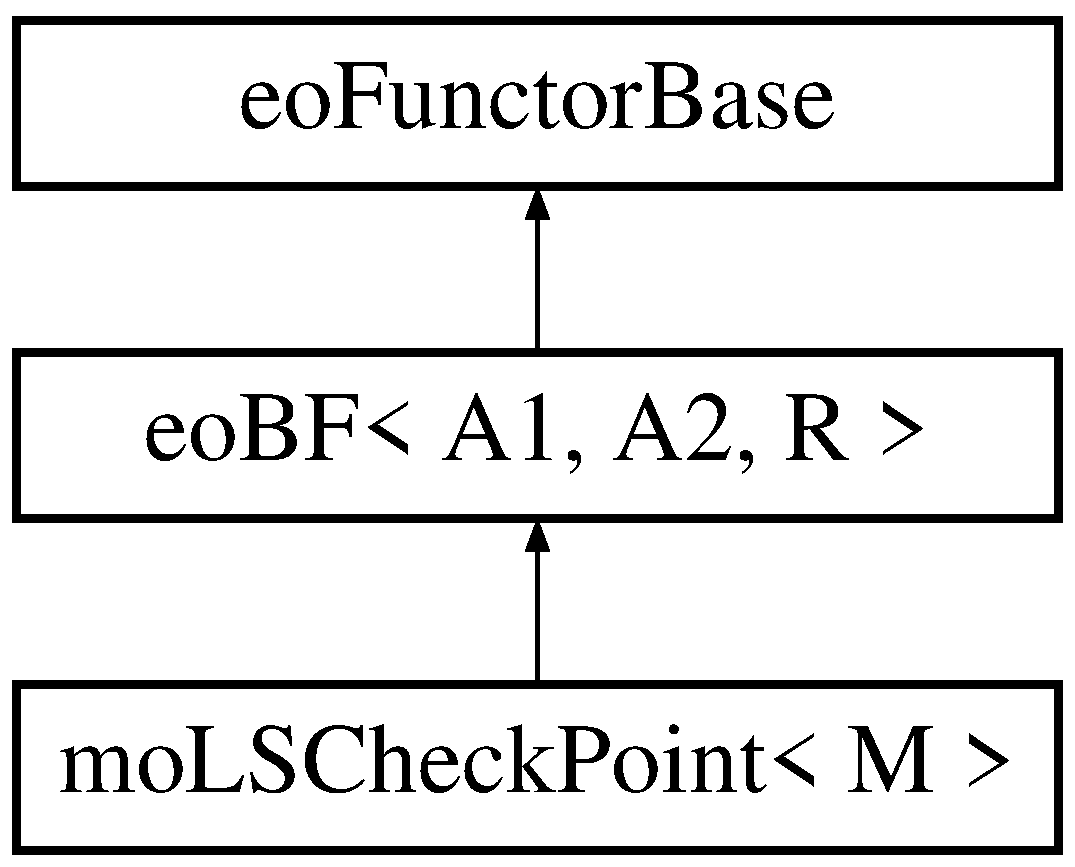
\includegraphics[height=3cm]{classmo_l_s_check_point}
\end{center}
\end{figure}
\subsection*{Public Member Functions}
\begin{CompactItemize}
\item 
void {\bf operator()} (const M \&\_\-move, const typename M::EOType \&\_\-solution)
\begin{CompactList}\small\item\em {\bf Function} which launches the checkpointing. \item\end{CompactList}\item 
void {\bf add} ({\bf eoBF}$<$ const M \&, const typename M::EOType \&, void $>$ \&\_\-function)
\begin{CompactList}\small\item\em Procedure which add a new function to the function vector. \item\end{CompactList}\end{CompactItemize}
\subsection*{Private Attributes}
\begin{CompactItemize}
\item 
std::vector$<$ {\bf eoBF}$<$ const M \&, const typename M::EOType \&, void $>$ $\ast$ $>$ {\bf functions}\label{classmo_l_s_check_point_56a7427a6aebac7955c22bab302c050a}

\begin{CompactList}\small\item\em Vector of functions. \item\end{CompactList}\end{CompactItemize}


\subsection{Detailed Description}
\subsubsection*{template$<$class M$>$ class moLSCheckPoint$<$ M $>$}

Class which allows a checkpointing system. 

Thanks to this class, at each iteration, additionnal function can be used (and not only one). 

Definition at line 46 of file moLSCheckPoint.h.

\subsection{Member Function Documentation}
\index{moLSCheckPoint@{moLSCheckPoint}!operator()@{operator()}}
\index{operator()@{operator()}!moLSCheckPoint@{moLSCheckPoint}}
\subsubsection{\setlength{\rightskip}{0pt plus 5cm}template$<$class M$>$ void {\bf moLSCheckPoint}$<$ M $>$::operator() (const M \& {\em \_\-move}, const typename M::EOType \& {\em \_\-solution})\hspace{0.3cm}{\tt  [inline]}}\label{classmo_l_s_check_point_e9b9d41e40dd7bab648327686b2b938d}


{\bf Function} which launches the checkpointing. 

Each saved function is used on the current move and the current solution.

\begin{Desc}
\item[Parameters:]
\begin{description}
\item[{\em \_\-move}]a move. \item[{\em \_\-solution}]a solution. \end{description}
\end{Desc}


Definition at line 57 of file moLSCheckPoint.h.

References moLSCheckPoint$<$ M $>$::functions.\index{moLSCheckPoint@{moLSCheckPoint}!add@{add}}
\index{add@{add}!moLSCheckPoint@{moLSCheckPoint}}
\subsubsection{\setlength{\rightskip}{0pt plus 5cm}template$<$class M$>$ void {\bf moLSCheckPoint}$<$ M $>$::add ({\bf eoBF}$<$ const M \&, const typename M::EOType \&, void $>$ \& {\em \_\-function})\hspace{0.3cm}{\tt  [inline]}}\label{classmo_l_s_check_point_f95f2dc556cdfbdc81688562ca95202d}


Procedure which add a new function to the function vector. 

The new function is added at the end of the vector. \begin{Desc}
\item[Parameters:]
\begin{description}
\item[{\em \_\-function}]a new function to add. \end{description}
\end{Desc}


Definition at line 72 of file moLSCheckPoint.h.

References moLSCheckPoint$<$ M $>$::functions.

The documentation for this class was generated from the following file:\begin{CompactItemize}
\item 
moLSCheckPoint.h\end{CompactItemize}
